\iffalse
\documentclass[journal,12pt,twocolumn]{IEEEtran}
\usepackage[none]{hyphenat}
\usepackage{graphicx}
\usepackage{listings}
\usepackage[english]{babel}
\usepackage{graphicx}
\usepackage{caption} 
\usepackage{amsmath}
\usepackage{hyperref}
\usepackage{booktabs}
\usepackage{array}
\usepackage{stix}


\title{\textbf{\\Line Assignment}}
\author{kanekal kousar}
\date{September 2022}

\providecommand{\norm}[1]{\left\lVert#1\right\rVert}
\providecommand{\abs}[1]{\left\vert#1\right\vert}
\let\vec\mathbf
\newcommand{\myvec}[1]{\ensuremath{\myvec{#1}}}
\newcommand{\mydet}[1]{\ensuremath{\begin{vmatrix}#1\end{vmatrix}}}
\providecommand{\brak}[1]{\ensuremath{\left(#1\right)}}

\begin{document}
\maketitle


\section{Question}
\textbf{\textit{Class 11, Exercise 10.1, Q(9):} 
\fi
Without using distance formula, show that points (– 2, – 1), (4, 0), (3, 3) and (–3, 2) are the vertices of a parallelogram.
	\begin{figure}[!ht]
		\centering
 \includegraphics[width=\columnwidth]{chapters/11/10/1/9/figs/paralellogram.png}
		\caption{}
		\label{fig:11/10/1/9}
  	\end{figure}
	\\
	\solution See Fig. 
		\ref{fig:11/10/1/9}.
\iffalse
}

\section{Solution}
\raggedright 

\begin{figure}[h!]
\centering
\includegraphics[scale=0.5]{fig/paralellogram.png}  
\caption{paralellogram ABCD}
\end{figure}

\vspace{0.25cm}
We can prove that the points are the vertices of a parallelogram if the direction vectors of opposite lines are equal

Consider  figure I,where
\fi


\begin{align}
\vec{A}=\myvec{-2 \\ -1  },  \vec{B}=\myvec{ 4\\ 0 }, 
\vec{C}=\myvec{3 \\ 3  },  \vec{D}=\myvec{-3 \\ 2  }
\end{align}
and
\begin{align}
	\vec{P} &=\vec{B}-\vec{A}=\myvec{6 \\ 1 \\ }
	\\
	\vec{Q}&=\vec{C}-\vec{D}=\myvec{6 \\ 1 \\ }
	\\
	\vec{R}&=\vec{A}-\vec{C}=\myvec{1 \\ -3 \\ }
	\\
	\vec{S}&=\vec{A}-\vec{D}=\myvec{1 \\ -3 \\ }
\end{align}
Since
$\vec{P}=\vec{Q}$
and 
$\vec{R}=\vec{S}$, from  
	  \eqref{eq:two-pgm},
$ABCD$ is a 
parallelogram
\iffalse

\section*{Construction}
\centering
\vspace{0.2cm}
{
\setlength\extrarowheight{2pt}
\begin{tabular}{|c|c|c|}
	\hline
	\textbf{Symbol}&\textbf{Value}&\textbf{Description}\\
	\hline
	A & $\myvec{-2 \\ -1 \\ }$ & Vertex A\\
	\hline
	B & $\myvec{4 \\ 0 \\ }$ & Vertex B\\
	\hline
	C &$\myvec{3 \\ 3 \\ }$ & Vertex C\\
	\hline
	D & $\myvec{-3 \\ 2 \\ }$ & Vertex D\\
	\hline
	P &$\myvec{1 \\ 6 \\ }$&vector AB\\
	\hline
	Q&$\myvec{1 \\ 6 \\ }$&vector DC\\
	\hline
	R&$\myvec{1 \\ -3 \\ }$&vector BC\\
	\hline
	S&$\myvec{1 \\ -3 \\ }$&vector AD\\
	\hline
\end{tabular}
}

\vspace{0.6cm}
Get the python code of the figures from
\begin{table}[h]
\large
\centering
\framebox{
\url{https://github.com/kkousar/KOUSAR_FWC/blob/main/line_assignment/code/line.py}}
\bibliographystyle{ieeetr}

\end{table}



\end{document}
\fi
